\iffalse
\chapter{2017}
\author{EE24BTECH11060}
\section{xe}
\fi
%\begin{enumerate}[start=14]
    \item During the experiment,the position of a fluid particle is monitoredby an instrument over a time period of $10$s.The trace of the particle given by the following figure represents a
    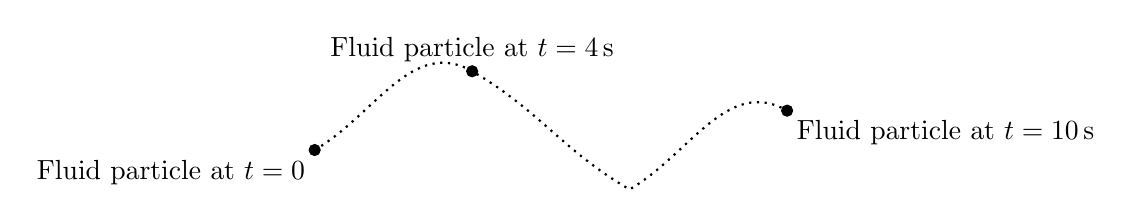
\begin{tikzpicture}
    % Draw the pathline as a dotted curve
    \draw[dotted, thick] (0,0) 
        to[out=30, in=150] (2,1) 
        to[out=-30, in=150] (4,-0.5)
        to[out=30, in=150] (6,0.5);

    % Draw points at specific times
    \filldraw (0,0) circle (2pt);
    \node[below left] at (0,0) {Fluid particle at $t = 0$};

    \filldraw (2,1) circle (2pt);
    \node[above] at (2,1) {Fluid particle at $t = 4 \, \mathrm{s}$};

    \filldraw (6,0.5) circle (2pt);
    \node[below right] at (6,0.5) {Fluid particle at $t = 10 \, \mathrm{s}$};

\end{tikzpicture}
    \begin{enumerate}
        \item streamline
        \item streakline
        \item pathline
        \item timeline
    \end{enumerate}
    \item In a cartesian two dimensional coordinate system ,$u$ and $v$ represent the velocities in $x$ and $y$ directions,respectively.For a certain flow,the velocity field is represented by the following expression:\\
    $V$=$\brak{ax+by}\hat{i}+\brak{cx+dy}\hat{j}$\\
    where the coefficients $a,b,c$ and $d$ are constants.For an incompressible flow,which one of the following relations is TRUE?
    \begin{enumerate}
        \item $a+d$=$0$
        \item $a+c$=$0$
        \item $b+d$=$0$
        \item $b+c$=$0$
    \end{enumerate}
    \item The stream function $\brak{\Psi}$ of a velocity field at any location $\brak{x,y}$ is gven as $\Psi$=$XY^2-2X^2Y^2$.What is the rate of rotation of the fluid element located at $\brak{2,2}$?
    \begin{enumerate}
        \item $8$
        \item $10$
        \item $12$
        \item $14$
    \end{enumerate}
    \item The nature of velocity profile within the laminar viscous sublayer in a turbulent pipe flow is
    \begin{enumerate}
        \item linear
        \item parabolic
        \item lagorithmic
        \item exponential
    \end{enumerate}
    \item In a $5$m vertical cylindrical tank,the water filled up to a height of $3$m from the bottom and the remaining space is filled wth oil of specific gravity $0.88$.Assume density od water as $1000\frac{kg}{m^3}$ and acceleration due to gravity to be $10\frac{m}{s^2}$.The gauge pressure ,rounded off to the first decimal place in $k\frac{N}{m^2}$,rounded off to the first decimal place, at a depth of $2.5$m from the top of the tank will be
    \item In a two-dimensional potential flow,a point source is located at the origin $\brak{x=0,y=0}$ as shown in the figure. The strength of the point source is $2$ $\frac{cm^2}{s}$.A uniform flow with velocity $1$$\frac{cm}{s}$ is approaching towards the point source at an angle $30\degree$ from the horizontal axis. What is the distance $\brak{cm}$ of the stagnation point in the flow field from the point source?
    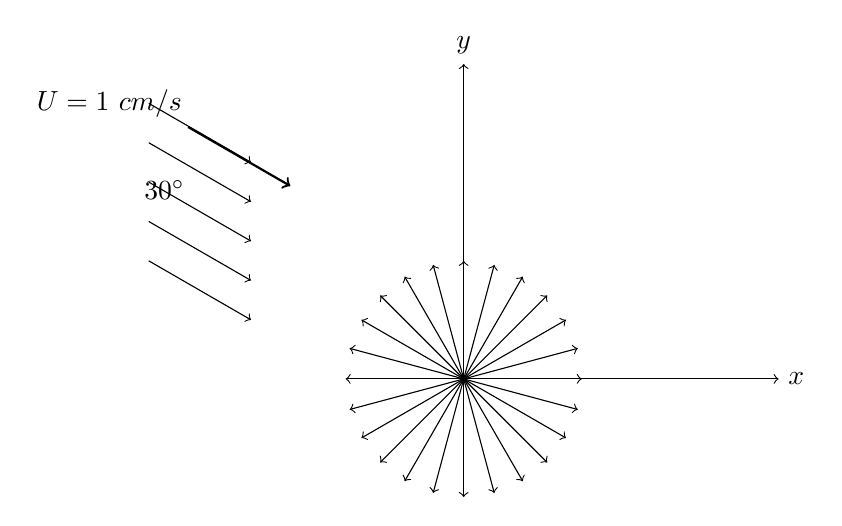
\begin{tikzpicture}
    \draw[->] (0,0) -- (4,0) node[right] {$x$};
    \draw[->] (0,0) -- (0,4) node[above] {$y$};

    \foreach \angle in {0,15,...,345} {
        \draw[->] (0,0) -- (\angle:1.5); 
    }

    \foreach \y in {1.5, 2, 2.5, 3, 3.5} {
        \draw[->] (-4, \y) -- ++(330:1.5);
    }
    \node at (-4.5,3.5) {$U = 1 \ \text{cm/s}$};

    \draw[->, thick] (-3.5,3.2) -- ++(330:1.5);
    \node at (-3.8,2.4) {$30^\circ$};

\end{tikzpicture}
    \item Two infinite parallel horizontal plates are separated by a small gap $\brak{d=20mm}$ as shown in the figure. The bottom plate is fixed and the gap between the plates is filled with oil having a density of $800$$\frac{kg}{m^3}$ and kinematic viscosity of $0.00033$$\frac{m^2}{s}$.Assume linear velocity profile between the plates and the oil  to be a Newtonian fluid.The shear stress $\brak{\frac{N}{m^2}}$ at the upper plate is\\ 
    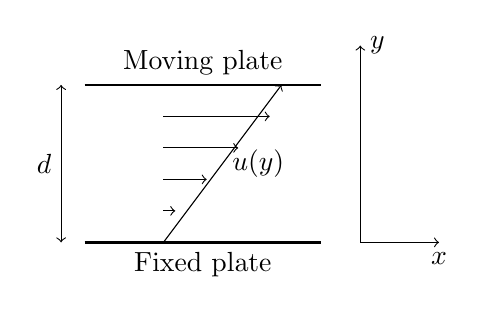
\begin{tikzpicture}
    % Plates
    \draw[thick] (-1,1) -- (2,1) node[above, pos=0.5] {Moving plate};
    \draw[thick] (-1,-1) -- (2,-1) node[below, pos=0.5] {Fixed plate};

    % Distance 'd'
    \draw[<->] (-1.3,-1) -- (-1.3,1) node[midway, left] {$d$};

    % Velocity profile u(y)
    \draw[->] (0,-1) -- (1.5,1) node[midway, right] {$u(y)$};
    \foreach \y in {-0.6,-0.2,0.2,0.6}{
        \draw[->] (0,\y) -- ({0.75+\y},\y);
    }

    % Coordinate system
    \draw[->] (2.5,-1) -- (2.5,1.5) node[right] {$y$};
    \draw[->] (2.5,-1) -- (3.5,-1) node[below] {$x$};
\end{tikzpicture}
    \item A spherical balloon of diameter $15$ m is supposed to lift a load of $3000$N.The lifting of load is achieved by heating the air inside the balloon. Assume, air to be an ideal gas and atmospheric preesure either outside or inside the balloon.The value of acceleration due to gravity is $9.81\frac{m}{s^2}$ and the values of temperature and the density of atmospheric air are $15^\circ C$ and $1.2\frac{kg}{m^3}$,respectively.In order to lift the specified load, the air inside the balloon should be heated to a temperature of $\brak{^\circ C}$ of    
    \item The velocity field in Cartesian coordinate system for a two-dimensional steady flow is given as:\\
    \begin{center}
        $\Bar{V}$=$\brak{\frac{V_{0}}{L}}\brak{x\hat{i}-y\hat{j}}$
    \end{center}
    where,$v_{0}$ and $L$ are constants.Which one of the following expressions represents the acceleration field $\Bar{a}$ for this flow?
    \begin{enumerate}
        \item $\Bar{a}$=$0$
        \item $\Bar{a}$=$\brak{\frac{V_{0}}{L}}\brak{x\hat{i}+y\hat{j}}$
        \item $\Bar{a}$=$\brak{\frac{V^2_{0}}{L^2}}\brak{x\hat{i}-y\hat{j}}$
        \item $\Bar{a}$=$\brak{\frac{V^2_{0}}{L^2}}\brak{x\hat{i}+y\hat{j}}$
    \end{enumerate}
    \item A cylindrical tank of $0.8$ m diameter is completely filled with water and its top surface is open to atmosphere as shown in the figure. Water is being discharged to the atmosphere from the circular hole of $15$ mm diameter located at the bottom of the tank. The value of acceleration due to gravity is $9.81$ $\frac{m}{s^2}$ How much time \brak{in seconds} would be required for water level to drop from the height of $1$ m to $0.5$ m?\\
    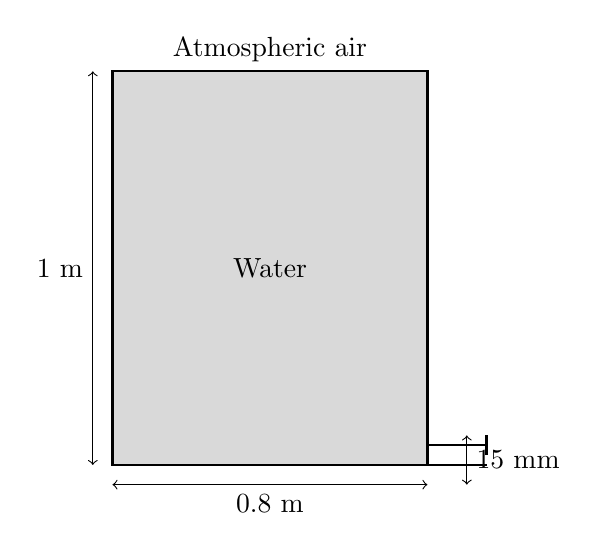
\begin{tikzpicture}[scale=0.5] % Adjust the scale factor to decrease the size

\fill[gray!30] (0,0) rectangle (8,10); % Water area
\node at (4,5) {Water};

\draw[thick] (0,0) rectangle (8,10); % Outer box

\draw[<->] (-0.5,0) -- (-0.5,10) node[midway, left] {1 m}; % Height label
\draw[<->] (0,-0.5) -- (8,-0.5) node[midway, below] {0.8 m}; % Width label

% Pipe segment at the bottom
\draw[thick] (8,0.5) -- (9.5,0.5); % Upper pipe segment
\draw[thick] (9.5,0.25) -- (9.5,0.75); % Pipe end
\draw[thick] (8,0) -- (9.5,0); % Lower pipe segment

% Dimension for pipe diameter
\draw[<->] (9,0.75) -- (9, -0.5) node[midway, right] {15 mm}; 

\node[above] at (4,10) {Atmospheric air}; % Atmospheric air label

\end{tikzpicture}

    \begin{enumerate}
        \item $188$
        \item $266$
        \item $376$
        \item $642$
    \end{enumerate}
 %\end{enumerate}
